% Packages

% Sets

% Formal statements


\begin{document}
\frame{\titlepage}

\begin{frame}{Computational complexity}
	
\includegraphics[width= 0.6\textwidth]{mario.png}

	\bigskip

	\pause
	We've used notation such as $O$ and $\Omega$ to describe the worst-case complexity of
	\emph{algorithms}. We must now turn to the complexity of \emph{computational problems}. 
\end{frame}

%

\begin{frame}{Computational complexity --- \emph{Church-Turing thesis and models of computation}}
	\textbf{Models of computation}
	\begin{itemize}
		\item Turing machines \checkmark (ISIS1106)
		\item RAM instructions \checkmark (Every other course)
		\item Lambda calculus
		\item Arithmetic circuits
		\item Boolean circuits
	\end{itemize}

	\bigskip

	\pause
	The \textbf{Church-Turing thesis} says that any two of these models are equivalent.

	\bigskip

	\pause
	Our discussion of computational complexity and so-called ``intractability'' will be in
	terms of the \emph{RAM} model of computation. 
\end{frame}

%

\begin{frame}{RAM instructions model of computation}
	\begin{itemize}
		\item We will use a \textbf{fixed programming language \underline{with types}},
			very Java-like.
		\item[] {\scriptsize \it *We may nonetheless occasionally discuss some statements
			in terms of Turing machines*}
	\end{itemize}
\end{frame}

%

\begin{frame}{Decision problems}
	\begin{defn}
		Let $\hat{X}$ be a type of our programming language and let
		$X \subset \hat{X}$. The \emph{decision problem} defined by $X$ consists
		of assigning \textbf{true} or \textbf{false} to the expression $x \in X$
		for all $x \in \hat{X}$. 
	\end{defn}

	\pause
	\begin{exl}
		\begin{enumerate}
			\item $\hat{X}= \ZZ$, $X=$ Primes.
			\item $\hat{X}= \mathtt{Graph}$, $X= \mathtt{connGraph}$. Namely,
				the problem of deciding whether or not a graph is
				connected.
			\item $\hat{X}= \mathtt{String}$, $X=$ Python programs that stop.
		\end{enumerate}
	\end{exl}

	\pause
	\textbf{Notation.} We will use $X \subset \hat{X}$ to denote the decision problem
	defined by $X$.
\end{frame}

%

\begin{frame}{Decision problems - computability}
	\begin{defn}
		The decision problem $X \subset \hat{X}$ is \emph{computable} if there
		exists a program
		\[
			\mathbf{boolean}\ \mathtt{checkX}(\hat{X}\ x)
		\]

		such that \(\mathtt{checkX}(x) =\) \textbf{true} if and only if
		$x \in X$.
	\end{defn}

	\pause
	\begin{exl}
		Examples 1 and 2 from the previous slide are computable, example 3 is
		not.
	\end{exl}
\end{frame}

%

\begin{frame}{Computable decision problems - Complexity classes}
	\begin{defn}
		The computable decision problem $X \subset \hat{X}$ is
		\emph{of class $P$} or is said to have \emph{polynomial time complexity}
		if there exists $k \in \Zpos$ such that
		\[
			\mathtt{checkX} \in O(n^k),
		\]
		where $n$ is the size of the input $x \in \hat{X}$.
	\end{defn}

	\pause
	\begin{exl}
		\begin{enumerate}
			\item The problem
				\(
					\text{Primes} \subset \ZZ \in P
				\)
				by taking \texttt{checkX} $=$ \texttt{isPrime} from the
				next slide.
			\item The problem 
				\(
					\mathtt{connGraph} \subset \mathtt{Graph} \in P
				\)
				by taking \texttt{checkX} $=$ \texttt{dfs}.
		\end{enumerate}
	\end{exl}
\end{frame}

%

\begin{frame}{Computable decision problems - Complexity classes}
	This primality test is based on Erathosthenes' theorem and Bolzano-Cauchy
	interpolation.

	\bigskip
	\lstinputlisting[language= Java, firstline= 3, lastline= 14]{Aula21.java}
\end{frame}

%

\begin{frame}{Computable decision problems - Complexity classes}
	\begin{defn}
		The computable decision problem $X \subset \hat{X}$ is
		\emph{of class $NP$} or is said to have
		\emph{non-deterministic polynomial time complexity} if there exist
		a type $Q$, a decision problem $Z \subset \hat{X} \times Q$, and a
		polynomial $p(n)$ satisfying the following conditions:
		\begin{enumerate}
			\item $x \in X$ if and only if there exists $q \in Q$ such that
				$(x, q) \in Z$.
			\item For all $(x, q) \in Z$ the size of $q$ is at most $p(n)$
				where $n$ is the size of $x$.
			\item \texttt{checkZ} is of class $P$.
		\end{enumerate}

		The decision problem $Z \subset \hat{X} \times Q$ is called a
		\emph{proof system} for $X \subset \hat{X}$.
	\end{defn}
\end{frame}

%

\begin{frame}{NP problems}
	\begin{exl}
		The problem
		\[
			\overline{\text{Primes}} \subset \ZZ
		\]
		of wheter or not a number is composite admits the proof system
		\[
			Z= \{(n, a) : 1 < |a| < |n|,\ \ n \ 
				\mathbf{mod}\ a = 0\}
		\]
		and
		\(
			Z \subset \ZZ \times \ZZ \in P
		\)
		since it consists of dividing $n$ by $a$.

		\bigskip
		\begin{qsn}
			The above argument about the proof system
			\(
				Z \subset \ZZ \times \ZZ
			\)
			only checks condition 3. Why does it also satisfy conditions 1 and 2? 
		\end{qsn}
	\end{exl}
\end{frame}

%

\begin{frame}
	\begin{defn}
		A graph is said to be \emph{Hamiltonian} if it contains a simple cycle.

		\bigskip
		\bigskip
		
		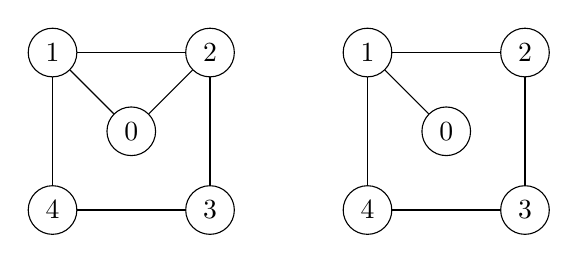
\begin{tikzpicture}
			% Hamiltonian example nodes
			\node[shape= circle, draw] (N1) at (0, 1) {1};
			\node[shape= circle, draw] (N2) at (2, 1) {2};
			\node[shape= circle, draw] (N3) at (2, -1) {3};
			\node[shape= circle, draw] (N4) at (0, -1) {4};
			\node[shape= circle, draw] (N0) at (1, 0) {0};
			% Hamiltonian example connections
			\draw (N0) -- (N1);
			\draw (N0) -- (N2);
			\draw (N1) -- (N2);
			\draw (N2) -- (N3);
			\draw (N3) -- (N4);
			\draw (N4) -- (N1);
			% Not hamiltonian example nodes
			\node[shape= circle, draw] (N1') at (4, 1) {1};
			\node[shape= circle, draw] (N2') at (6, 1) {2};
			\node[shape= circle, draw] (N3') at (6, -1) {3};
			\node[shape= circle, draw] (N4') at (4, -1) {4};
			\node[shape= circle, draw] (N0') at (5, 0) {0};
			% Not hamiltonian example connections
			\draw (N0') -- (N1');
			\draw (N1') -- (N2');
			\draw (N2') -- (N3');
			\draw (N3') -- (N4');
			\draw (N4') -- (N1');
		\end{tikzpicture}
	\end{defn}
\end{frame}

\begin{frame}{NP problems - HamD}
	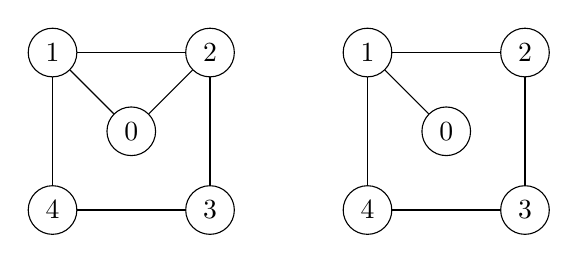
\begin{tikzpicture}
		% Hamiltonian example nodes
		\node[shape= circle, draw] (N1) at (0, 1) {1};
		\node[shape= circle, draw] (N2) at (2, 1) {2};
		\node[shape= circle, draw] (N3) at (2, -1) {3};
		\node[shape= circle, draw] (N4) at (0, -1) {4};
		\node[shape= circle, draw] (N0) at (1, 0) {0};
		% Hamiltonian example connections
		\draw (N0) -- (N1);
		\draw (N0) -- (N2);
		\draw (N1) -- (N2);
		\draw (N2) -- (N3);
		\draw (N3) -- (N4);
		\draw (N4) -- (N1);
		% Not hamiltonian example nodes
		\node[shape= circle, draw] (N1') at (4, 1) {1};
		\node[shape= circle, draw] (N2') at (6, 1) {2};
		\node[shape= circle, draw] (N3') at (6, -1) {3};
		\node[shape= circle, draw] (N4') at (4, -1) {4};
		\node[shape= circle, draw] (N0') at (5, 0) {0};
		% Not hamiltonian example connections
		\draw (N0') -- (N1');
		\draw (N1') -- (N2');
		\draw (N2') -- (N3');
		\draw (N3') -- (N4');
		\draw (N4') -- (N1');
	\end{tikzpicture}
	\begin{exl}
		The problem
		\(
			\mathtt{Ham} \subset \mathtt{Graph}
		\)
		admits the proof system
		\[
			Z= \{(g, \mathbf{u}) : B(g, \mathbf{u})\} \subset
			\mathtt{Graph} \times \ZZ\texttt{[$\,$]}
		\]
		where $B(g, \mathbf{u})$ is \textbf{true} if and only if
		\(
			\mathbf{u}= [u_0, \ldots, u_{n-1}]
		\)
		is a sequence of nodes in $g$ such that 
		\(
			\{u_i, u_{(i+1)\ \mathbf{mod}\ n}\} \in A_g
		\)
		for $i = 0, \ldots, n-1$.
	\end{exl}
\end{frame}

%

\begin{frame}{NP problems - HamD}
	\(
		Z \subset \mathtt{Graph} \times \ZZ\texttt{[\,]} 
	\)
	from the previous slide is a proof system for \texttt{Ham} $\subset$
	\texttt{Graph} because
	\begin{enumerate}
		\item Simple cycles on a graph can be represented with valid
			non-repeating sequences of nodes.
		\item For each
			\(
				(g, \mathbf{u}) \in Z
			\)
			we have $|\mathbf{u}| \in O(|g|)$.
		\item \texttt{checkZ} is $O(n)$ because it scans \textbf{u} to check
			if it corresponds to an edge sequence that defines a cycle.
	\end{enumerate}

	\bigskip

	\textbf{Notation.} We use \texttt{HamD}, read as ``\emph{Hamiltonian decision}'',
	to denote the decision problem \texttt{Ham} $\subset$ \texttt{Graph}.
\end{frame}

%

\begin{frame}
	\begin{defn}
		Let $G= (N, A)$ be an undirected graph. A \emph{cover} of $G$ is a
		subset $N' \subset N$ such that $a \cap N' \neq \emptyset$ for all
		$a \in A$.
	\end{defn}
\end{frame}

%

\begin{frame}{NP problems - CovD}
	\begin{defn}
		Let
		\[
			\begin{array}{l}
				\hat{X}= \mathtt{Graph} \times \ZZ\ \mbox{ and let}\\
				X=
				\{
					(g, k) |\ \mbox{$g$ has a cover of size $k$}
				\}. 
			\end{array}
		\]

		We then call
		\(
			X \subset \hat{X}
		\)
		the \emph{cover decision problem} and denote it by \texttt{CovD}.
	\end{defn}

	\bigskip
	It is of class $NP$ because it admits a proof system
	\(
		Z \subset \hat{X} \times \ZZ\texttt{[\,]}
	\)
	given by
	\[
		Z=
		\{
			((g,k), \mathbf{u}) |\ 
			\mbox{$\mathbf{u}$ defines a cover of $g$ of size $k$}
		\}
	\]
\end{frame}

%

\begin{frame}{Quiz - 15 min}
	\centering
	
\includegraphics[width= 0.3\textwidth]{marcela.png}

	\bigskip

	\pause
	
	\raggedright
	Demuestre que $Z$ satisface las propiedades de un sistema de pruebas para
	\texttt{CovD}.
\end{frame}

%

\begin{frame}{Reductions}
	\begin{defn}
		We say that the problem
		\(
			X \subset \hat{X}
		\)
		is \emph{polynomial time reducible} to the problem
		\(
			Y \subset \hat{Y}
		\)
		if there exists an algorithm
		\[
			\hat{Y} \ \mathtt{translate}(\hat{X} \ x)
		\]
		such that
		\begin{enumerate}
			\item
				\(
					\tau_{\mathtt{translate}} \in O(n^k)
				\)
				for some $k \in \Zpos$ where $n= |x|$.
			\item
				\(
					X = \mathtt{translate}^{-1}(Y).
				\)	  
		\end{enumerate}

		We will denote this by
		\[
			X \subset \hat{X} \leq_P Y \subset \hat{Y}
		\]
		and simply say \emph{reducible} instead of ``polynomial time reducible''.
	\end{defn}
\end{frame}

%

\begin{frame}{Reductions}
	\begin{thm}
		\begin{enumerate}
			\item 
				\(
					\mathtt{CovD} \leq_P \mathtt{HamD}
				\) (Hard). \pause
			\item 
				\(
					\mathtt{HamD} \leq_P \mathtt{TSPD}
				\) (Easy).
		\end{enumerate}
	\end{thm}
\end{frame}
\end{document}
